\documentclass[article]{ajs}

%%%%%%%%%%%%%%%%%%%%%%%%%%%%%%
%% declarations for jss.cls %%%%%%%%%%%%%%%%%%%%%%%%%%%%%%%%%%%%%%%%%%
%%%%%%%%%%%%%%%%%%%%%%%%%%%%%%
 
\usepackage{etoolbox}
 
 
%% almost as usual
\author{Matthias Medl\,\orcidlink{0000-0002-3354-4579}\\ Institute of Statistics \\ BOKU University \\ Vienna \And 
        Dianne Cook\,\orcidlink{0000-0002-3813-7155}\\ Monash Data Futures Institute \\ Monash University \\ Melbourne \And
        Ursula Laa\,\orcidlink{0000-0002-0249-6439}\\ Institute of Statistics \\ BOKU University \\ Vienna}
%% \AND can be used instead of \And and starts a new line
\title{pytourr: Interactive Visualization Interface for the tourr Package}

%% for pretty printing and a nice hypersummary also set:
\Plainauthor{Matthias Medl, Dianne Cook, Ursula Laa} %% comma-separated
\Plaintitle{pytourr: Interactive Visualization Interface for the tourr Package} %% without formatting
\Shorttitle{pytourr} %% a short title (if necessary)

%% an abstract and keywords
\Abstract{
This guidelines are tested for new versions of texlive and current version of overleaf's LaTeX version. 
%If you run into problems using ealier versions of texlive, please report to \email{matthias.templ@gmail.com}. 

  This template and guide of the Austrian Journal of Statistics (AJS) shows the required style of manuscripts submitted to the Austrian Journal of Statistics. We strongly recommend
to follow the given instructions exactly already when writing the paper. When submitting papers to AJS, it is essential to follow these guidelines. The present document can be used directly as a template. The file with the name \texttt{guidelinesAJS.tex} can be obtained from the following website \href{https://github.com/matthias-da/ajs-public}{https://github.com/matthias-da/ajs-public}, or directly as overleaf template in their academic journal section. 

Manuscripts submitted without consideration of the AJS style guide will most likely not be forwarded for review, but rejected with the possibility of resubmission.
}
\Keywords{interactive visualization, tourr, exploratory data analysis, \proglang{R}, \proglang{python}}
\Plainkeywords{keywords, comma-separated, non-capitalized,, R} %% without formatting
%% at least one keyword must be supplied

%% publication information
%% NOTE: Typically, this can be left commented and will be filled out by the technical editor
%% \Volume{50}
%% \Issue{9}
%% \Month{June}
%% \Year{2012}
%% \Submitdate{2012-06-04}
%% \Acceptdate{2012-06-04}
%% \setcounter{page}{1}
\Pages{1--xx}

%% The address of (at least) one author should be given
%% in the following format:
\Address{
  Matthias Templ\\
  Institue of Data Analysis and Process Design\\
  University of Applied Sciences and Arts Northwestern Switzerland\\
  CH-4600 Olten, Switzerland\\
  E-mail: \email{matthias.templ@gmail.com}\\
  URL: \url{https://www.fhnw.ch/de/personen/matthias-templ}
}
%% It is also possible to add a telephone and fax number
%% before the e-mail in the following format:
%% Telephone: +43/512/507-7103
%% Fax: +43/512/507-2851

%% for those who use Sweave please include the following line (with % symbols):
%% need no \usepackage{Sweave.sty}

%% end of declarations %%%%%%%%%%%%%%%%%%%%%%%%%%%%%%%%%%%%%%%%%%%%%%%


\begin{document}

%% include your article here, just as usual

Before we look at style in more detail, the most common mistakes and errors are described:

\section{Comments on frequently made mistakes and concerns}

To avoid a reject in first place:

\begin{description}
\item[C1.word] Do not submit articles written with prohibited software like Microsoft Word or similar WYSWYG software. We like to send your manuscript with the AJS style to reviewers. 
\item[C1.conclusion] Write a conclusion and/or discussion discussing your results.  Discuss how your method improved science and give value to the community, and discuss differences to other alternative methods. 
\item[C1.data.documentation] Give sufficient documentation on data you are using.
\item[C1.application] In case you have numerical examples, use convincing applications and interesting data. Do not use \texttt{toy} data with 50 observations and no explanatory variables / covariables, for example. 
\end{description}

To do justice to the style from the very beginning:

\begin{description}
\item[C2.title] Title in Capitalized Style. See the title of the guidelines for illustration.
\item[C2.subsections]  Subsection in lower case style. See the subsection of the guidelines for illustration
\item[C2.references]  Captialized Title for references. E.g. \cite{fleet20} should appear in the reference list as ``Fleet Management in Free-Floating Bike Sharing Systems Using
  Predictive Modelling and Explorative Tools.'' and NOT as ``Fleet management in free-floating bike sharing systems using
  predictive modelling and explorative tools.''.
\item[C2.doi]  Include DOI numbers for each citation (if possible)
\item[C2.graphics]  Use vector-based graphics such as \texttt{pdf}. Do not use pixel-based graphics like \texttt{png}, \texttt{jpeg}, and do not convert from \texttt{png} or \texttt{jpeg} to \texttt{pdf}
\item{C2.tables} Produce tables in \LaTeX{}. (no screenshots)
\end{description}

\section{Introduction}


The style file of the Austrian Journal of Statsitics is based on the style file of the Journal of Statistical Software (JSS) including minor modifications. We thank Achim Zeileis for his great work on the JSS style file.

The Austrian Journal of Statistics is freely available over the net. Free and open-source tools used for production of your manuscript are therefore also highly supported. Code to reproduce the figures and tables in manuscripts as well as methods implemented in software can be published as supplementary material. This increases usually the number of 
downloads of your article.

After review, final sources can also be sent as \texttt{knitr} \citep{knitr} .Rnw file.

%Graphics should be inserted as PostScript files using the
%package {\tt psfig} or {\tt graphicx}. Bibliographic references
%should be given using {\tt bibtex} in the {\em author-date\/}
%style.


\section{Writing your manuscript}

In order to obtain a uniform layout and to ease the production as
much as possible it is highly recommended to use \LaTeXe\ for the
text processing. 


Technically, you have three possibilities to choose the software for writing your manuscript:

- Select from the overleaf template for academic journals the template for the Austrian Journal of Statistics.
- Download the template from \href{https://github.com/matthias-da/ajs-public}{https://github.com/matthias-da/ajs-public}
- use the R package \texttt{rtcles}, function \texttt{ajs\_article}.
- use the overleaf template for the Austrian Journal of Statistics, found online at \href{https://www.overleaf.com/latex/templates/tagged/academic-journal}{https://www.overleaf.com/latex/templates/tagged/academic-journal}



Each article must have a summary in English which
inform the reader quickly on the contents and the substantial
results. The length surely depends on the contents. 
Mathematical formulas and references should be
avoided in the summary.

Headings and footings as well as pagination will be added during
the production. Footnotes should be avoided.

The article should be structured by enumerated sections and
subsections. The title should be in title case style, sections and subsections in section case style. Graphics and tables must contain captions, above
tables and below graphics (figures). Examples are (see Figure~\ref{fig:Fig3.4} and Table~\ref{Tab3.4}).
Graphics \textbf{should be produced in \textbf{pdf} format} and included 
 at suitable places of the manuscript. 

\begin{figure}[hbt]
\begin{center}
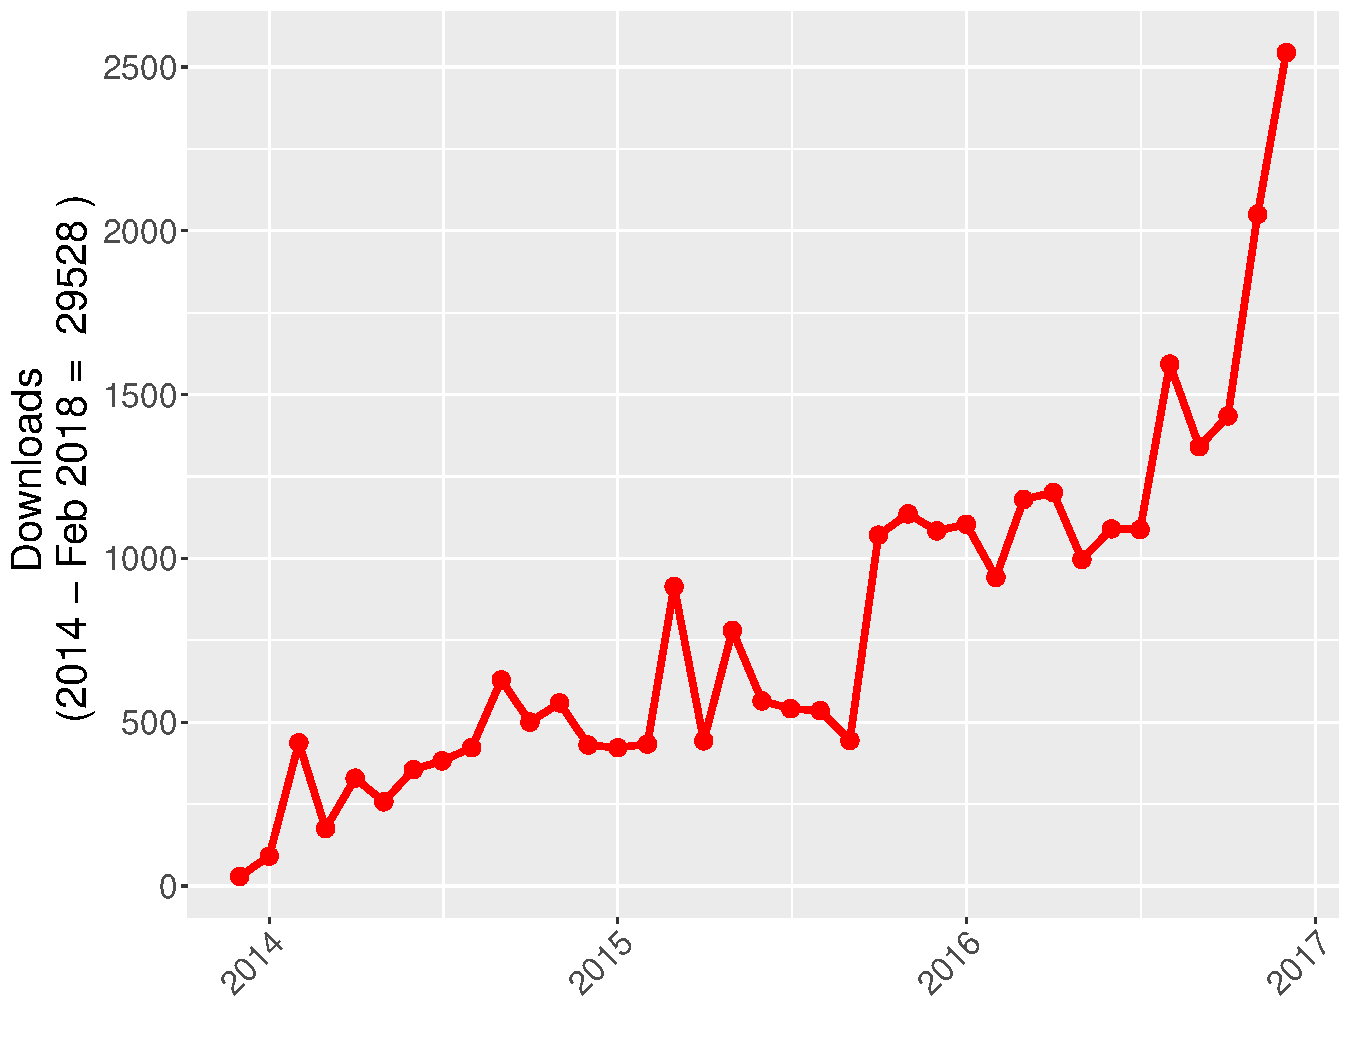
\includegraphics{ajs-download20180210}
\caption{\label{fig:Fig3.4}Download statistics of articles per month at the Austrian Journal of Statistics.}  
\end{center}
\end{figure}

\begin{table}[hbt]
\caption{\label{Tab3.4}80 measured values of access time.}
\vspace*{-5mm}
\small
\hspace{1.5cm}
\begin{center}
\begin{tabular}{|llllllll|}
\toprule
70.0 & 68.6 & 67.9 & 66.3 & 71.0 & 64.2 & 69.6 & 71.0\\
... & ... & ... & ... & ... & ... & ... & ...\\
%69.7 & 69.0 & 73.4 & 69.0 & 70.1 & 69.8 & 69.0 & 73.0\\
%70.0 & 69.1 & 69.5-& 67.9 & 72.8 & 72.1 & 69.5+& 70.1\\
%70.2 & 69.1 & 68.9 & 68.3 & 74.9 & 68.4 & 69.1 & 66.6\\
%71.1 & 69.2 & 71.2 & 68.9 & 70.9 & 70.6 & 69.9 & 69.9\\
%69.4 & 69.5+& 68.5+& 70.9 & 71.6 & 68.9 & 72.0 & 70.3\\
%68.6 & 68.5-& 67.8 & 72.2 & 68.7 & 70.6 & 66.9 & 69.3\\
%71.4 & 68.7 & 74.2 & 68.8 & 71.4 & 71.8 & 67.5-& 70.4\\
%71.4 & 67.4 & 69.5-& 72.4 & 70.4 & 69.3 & 68.2 & 67.0\\
71.7 & 70.5+& 72.5-& 68.2 & 67.6 & 68.6 & 70.5-& 65.8\\
\bottomrule
\end{tabular}
\end{center}
\end{table}

Mathematical formulas should be enumerated as far as they are
referenced \textbf{only}. E.g.~Equation~(\ref{form3.1}) shows the density 
\begin{equation}\label{form3.1}
f(x) =
\frac1{\sqrt{2\pi}\sigma}e^{-\frac{(x-\mu)^2}{2\sigma^2}}\,.
\end{equation}

Please consider 

\begin{itemize}
\item  capitalized title case for titles and for all references and 
\item sentence, non-capitalized case for sections and subsections.
\end{itemize}


Cited literature should be summarized at the end of the article in
form of a non-enumerated section. \cite{knitr} is a reference
to an article. If the citation is in parentheses, it
should look like \citep{knitr}. The latter verison is used for indirect citations while the first one to directly cite an article.
References should be in title case.

Correspondence addresses of author(s) should be added at the end
of the manuscript. 


\section{Submission and refereeing}


\subsection{Submission}

Consideration of the previously stated rules are of great help for
the editing process. Whenever technically possible, manuscripts
should be submitted through the editorial system at \href{www.ajs.or.at}{www.ajs.or.at}. The authors must be registered at this website.

\subsection{Refereing}

All contributions will be anonymously refereed. Cited literature which is
hardly available should accompany the submitted manuscript. It
should also be considered to place used and analyzed data at
disposal for the referees (if there are no legal or technical
arguments against).

Editor and referees must trust that the contribution has not been
submitted for publication at the same time at another place. It is
fair that the submitting author notifies if an earlier version has
already been submitted somewhere before.

\subsection{Copyrights and fees}

The Austrian Journal of Statistics is free of
charge. Generally, we use the Creative Commons Attribution License (CC-BY).

For copyright issues, publication ethics and malpractice statements, please have a look at 
\href{www.ajs.or.at}{www.ajs.or.at}


\section{Checklist}

We list the most common mistakes when submitting manuscripts to the journal and formulate them in form of questions.

\begin{itemize}
\item Did you upload a pdf of your manuscript for review? (no Word, no .tex, ...)
\item Did you use the style of AJS?  
\item Are your graphics produced in pdf format? 
\item Is your title captialized?
\item Are the titles of your cited papers in your references capitalized?
\item Are your section and subsection headers non-capitalized form?
\item Are your tables produced with \LaTeX ? (no screenshots)
\item Have you cited the software you used, e.g. R itself and R packages used? To not cite software is plagiarism and violates intellectual properties of the authors of the software.
\item Did you proposed at least three independent reviewers?
\end{itemize}

\section{Frequently asked questions}

\noindent 
\begin{enumerate}
\item \textit{My citation shows all authors and not the typically shown et al.}. \\ Answer: this is ok. We like to show all authors in the text.
\item \textit{When I submit a paper, how long does it take to be published} \\ Answer: The average time from submission to publication is approx. 132 days. But it heavily depends if you can make satisfying revisions in time. 
\item \textit{In which databases is AJS indexed.} \\
Answer: we are indexed in many of them, most notable is Scopus (from Elsevier). More information can be found at the website of AJS. 
\item \textit{Can I upload my paper on \href{https://arxiv.org/}{https://arxiv.org/} and distribute before the paper is online at AJS? } \\
Answer: Of course, you can do it. However, please clearly point out in the header of the paper that this paper is under review in the Austrian Journal of Statistics and will likely be published there. Note that the readers should check if the paper is already be published at AJS for correct citation, i.e. finally the journal should be cited. Update and upload  \href{https://arxiv.org/}{https://arxiv.org/} or similar sites with the final version in AJS style after the paper is published  in AJS. 

\end{enumerate}

\section{Known issues}

While in the documentclass arcticle a section header with special characters works without problems, e.g. \verb|\section{A \& B}|, this results in an error in the documentclass ajs. The solution is \verb|\section[A and B]{A \& B}|.


%\bibliographystyle{plainat}
\bibliography{template-guidelinesAJS}



\end{document}